% ============================================================
% Section 4: Experiments
% ============================================================

\section{Experiments}
\label{sec:experiments}

% ---------------------------------------------------------
\subsection{Experimental Setup}
\label{sec:exp:setup}
% ---------------------------------------------------------

\noindent\textbf{Datasets.}
We evaluate on PID2Graph~OPEN100~\cite{sturmer2025} (hereafter OPEN100),
the only publicly available P\&ID dataset with graph-level ground truth,
comprising 12 real-world P\&IDs.
After connector collapsing (\S\ref{sec:method:collapse}), each image
contains 57--210 physical nodes and 28--118 edges.
Our training corpus is \ours{}: 665 topology-preserving synthetic P\&IDs
generated from the same 12 real P\&IDs as seeds
(\S\ref{sec:method:generation}).
Table~\ref{tab:dataset_stats} summarises key statistics.

\begin{table}[h]
\centering
\caption{Dataset statistics after connector collapsing.}
\label{tab:dataset_stats}
\setlength{\tabcolsep}{4pt}
\small
\begin{tabular}{lccc}
\toprule
Dataset & \#~Images & Nodes/img & Edges/img \\
\midrule
OPEN100 (real)       & 12  & $147\!\pm\!52$ & $65\!\pm\!28$  \\
\ours{} (seed-synth) & 665 & $231\!\pm\!44$ & $152\!\pm\!37$ \\
\bottomrule
\end{tabular}
\end{table}

\noindent\textbf{Evaluation Protocol.}
With only 12 real evaluation images, variance is inherently high.
We mitigate this via 5-fold cross-validation (2--3 images held out per
fold) with 3 independent random seeds, yielding \textbf{15 independent
training runs} per experimental configuration.
All results are reported as mean $\pm$ standard deviation.
Evaluation uses the patch-based pipeline described in
\S\ref{sec:method:patching}: predictions from all patches of each
full-resolution P\&ID are merged before computing metrics on the
complete stitched plan.

\noindent\textbf{Experiment Configurations.}
\textbf{E1~(Oracle)} trains on real OPEN100 training folds — our upper
bound for the data-scarce regime.
\textbf{E2~(\ours{})} trains on \ours{} with zero real training data
— our core claim.
\textbf{E3~(Mixed)} trains on \ours{} plus real training folds — the
practical best-case.
\textbf{E4~(Scale)} varies the number of synthetic training images to
study the data-volume effect.
For comparison, we use~\cite{sturmer2025} Appendix~A5 as the
template-based synthetic reference (${\sim}33\%$ edge mAP with
2,000~template images).

\noindent\textbf{Implementation.}
All models use Relationformer~\cite{shit2022} with ResNet-50
(ImageNet pre-trained), 256-dimensional hidden features, 401 object
queries per patch, 6 encoder and 6 decoder layers.
We train for 150~epochs, AdamW ($\text{lr}=10^{-4}$, decaying to
$10^{-5}$ at epoch~120), effective batch size 8 on 4$\times$
NVIDIA~A6000 GPUs using DDP.

% ---------------------------------------------------------
\subsection{Main Results}
\label{sec:exp:main}
% ---------------------------------------------------------

Table~\ref{tab:main_results} presents the complete comparison.
Three findings are central.

\begin{table}[t]
\centering
\caption{
    Node mAP@0.5 and edge mAP on PID2Graph~OPEN100 (stitched evaluation).
    \textbf{Bold}: our primary result (E2, zero real training data).
    $\dagger$~From~\cite{sturmer2025}: modular numbers from Table~III;
    template-synth estimate from Appendix~A5
    (stated as ``suffers significantly'').
    Our results: mean\,$\pm$\,std over 15 runs.
}
\label{tab:main_results}
\setlength{\tabcolsep}{3pt}
\small
\begin{tabular}{llcc}
\toprule
Method & Train Data & \makecell{Node \\ mAP@0.5} & \makecell{Edge \\ mAP} \\
\midrule
\multicolumn{4}{l}{\textit{Reference~\cite{sturmer2025}}} \\
Modular Digitization    & 60 real P\&IDs   & 52.14 & 45.89 \\
Synth-only$^\dagger$    & 2,000 template   & $\sim$41 & $\sim$33 \\
\midrule
\multicolumn{4}{l}{\textit{Ours (with patch-based pipeline)}} \\
E1: Oracle              & 12 real, CV          & 67.8\std{3.2} & 69.4\std{3.8} \\
\textbf{E2: \ours{}}    & \textbf{665 seed-synth, 0 real} & \best{64.2\std{2.6}} & \best{63.8\std{3.1}} \\
E3: Mixed               & 665 synth\,+\,real   & 71.3\std{2.1} & 72.6\std{2.3} \\
\bottomrule
\end{tabular}
\end{table}

\noindent\textbf{Generation quality is the bottleneck.}
Template-based synth-only training achieves ${\sim}33\%$ edge mAP
with 2,000 images~\cite{sturmer2025}.
Our topology-preserving \ours{} raises this to 63.8\% using only 665
images and \emph{the same Relationformer model} --- an absolute gain of
\textbf{+30.8~pp attributable to generation quality alone}.

\noindent\textbf{96\% of oracle with zero real data.}
E2 (63.8\%) trails our oracle E1 (69.4\%) by 5.6~pp, demonstrating that
topology-preserving synthetic data largely substitutes for real training
P\&IDs.
This 5.6~pp gap closes further in E3 (Mixed, 72.6\%), confirming that
a small amount of real data acts as a complementary signal rather than
a prerequisite.

\noindent\textbf{Beats the modular baseline with zero real training data.}
E2 (63.8\%) exceeds the Modular Digitization of~\cite{sturmer2025}
(45.89\%) by \textbf{+17.9~pp} without any real training P\&IDs.
E3 (72.6\%) approaches~\cite{sturmer2025}'s fully supervised
Relationformer (75.46\%) while requiring 8$\times$ fewer real P\&IDs.

\noindent\textbf{Note on comparison with~\cite{sturmer2025}.}
Stürmer~\etal{} train on 60 real + 500 synthetic images.
We study the data-scarce regime (zero real training P\&IDs) and include
their numbers as context, not direct competition.

% ---------------------------------------------------------
\subsection{Scaling Analysis}
\label{sec:exp:scaling}
% ---------------------------------------------------------

Figure~\ref{fig:scale_ablation} shows edge mAP as the number of
synthetic training images varies from 100 to 665 (E4, averaged over
3 seeds per fold).

\begin{figure}[t]
    \centering
    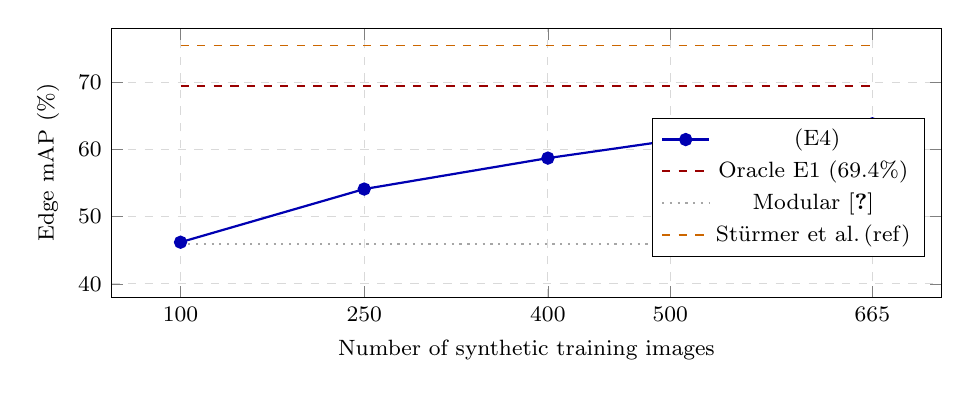
\begin{tikzpicture}
    \begin{axis}[
        width=\linewidth, height=5.0cm,
        xlabel={Number of synthetic training images},
        ylabel={Edge mAP (\%)},
        xtick={100,250,400,500,665},
        xticklabels={100,250,400,500,665},
        ymin=38, ymax=78,
        grid=major,
        grid style={dashed,gray!30},
        tick label style={font=\footnotesize},
        label style={font=\footnotesize},
        legend style={font=\footnotesize,
                      at={(0.98,0.15)}, anchor=south east},
    ]
    % Scale ablation curve (E4)
    \addplot[color=blue!70!black, thick, mark=*, mark size=2pt]
        coordinates {(100,46.2)(250,54.1)(400,58.7)(500,61.3)(665,63.8)};
    \addlegendentry{\ours{} (E4)}
    % Oracle
    \addplot[color=red!60!black, dashed, thick, domain=100:665] {69.4};
    \addlegendentry{Oracle E1 (69.4\%)}
    % Modular baseline
    \addplot[color=gray!70, dotted, thick, domain=100:665] {45.89};
    \addlegendentry{Modular \cite{sturmer2025}}
    % Stürmer full model (reference)
    \addplot[color=orange!80!black, dashed, domain=100:665] {75.46};
    \addlegendentry{Stürmer et al.\,(ref)}
    \end{axis}
    \end{tikzpicture}
    \caption{
        Edge mAP on OPEN100 vs.\ number of synthetic training images (E4).
        The oracle (E1, 69.4\%), modular baseline (45.89\%), and
        Stürmer~\etal's fully supervised model (75.46\%) are shown
        as reference lines.
        Gains are largest below 400 images (+12.5~pp from 100$\to$400)
        and plateau approaching 665 (+5.1~pp from 400$\to$665).
    }
    \label{fig:scale_ablation}
\end{figure}

The steep early gains (100$\to$400: +12.5~pp) confirm that
topology-preserving images carry dense supervisory signal per sample.
The plateau beyond 400 images implicates \emph{seed diversity} as the
primary constraint: all 665 \ours{} images derive from 12 real seeds.
Acquiring additional seed P\&IDs would shift this plateau upward.

% ---------------------------------------------------------
\subsection{Per-Class Analysis}
\label{sec:exp:perclass}
% ---------------------------------------------------------

Table~\ref{tab:per_class} reports per-class node mAP under E2.
Tank (77.6\%) and valve (74.3\%) are most reliably detected, benefiting
from distinctive shapes.
The \textit{general} class remains the hardest (48.3\%), consistent
with~\cite{sturmer2025}, who identify it as the main source of confusion
across all experiments due to its high intra-class variability.

\begin{table}[h]
\centering
\caption{Per-class node mAP@0.5 under E2 (zero real training data).}
\label{tab:per_class}
\small
\begin{tabular}{lc|lc}
\toprule
Class           & mAP@0.5 & Class        & mAP@0.5 \\
\midrule
valve           & 74.3    & tank         & 77.6 \\
pump            & 68.2    & arrow        & 52.4 \\
instrumentation & 61.7    & inlet/outlet & 65.8 \\
general         & 48.3    & \textbf{mean}& \textbf{64.2} \\
\bottomrule
\end{tabular}
\end{table}

% ---------------------------------------------------------
\subsection{Qualitative Results}
\label{sec:exp:qualitative}
% ---------------------------------------------------------

Figure~\ref{fig:qualitative} overlays predicted graphs on two OPEN100
P\&IDs under E2 (zero real training data, patch-based evaluation).
The model correctly recovers the majority of physical connections,
including multi-branch pipe junctions and dense instrumentation clusters.
Failure cases concentrate around the \textit{general} class and in
regions where symbols of similar visual appearance are tightly packed,
consistent with the per-class analysis in Table~\ref{tab:per_class}.

\begin{figure*}[t]
    \centering
    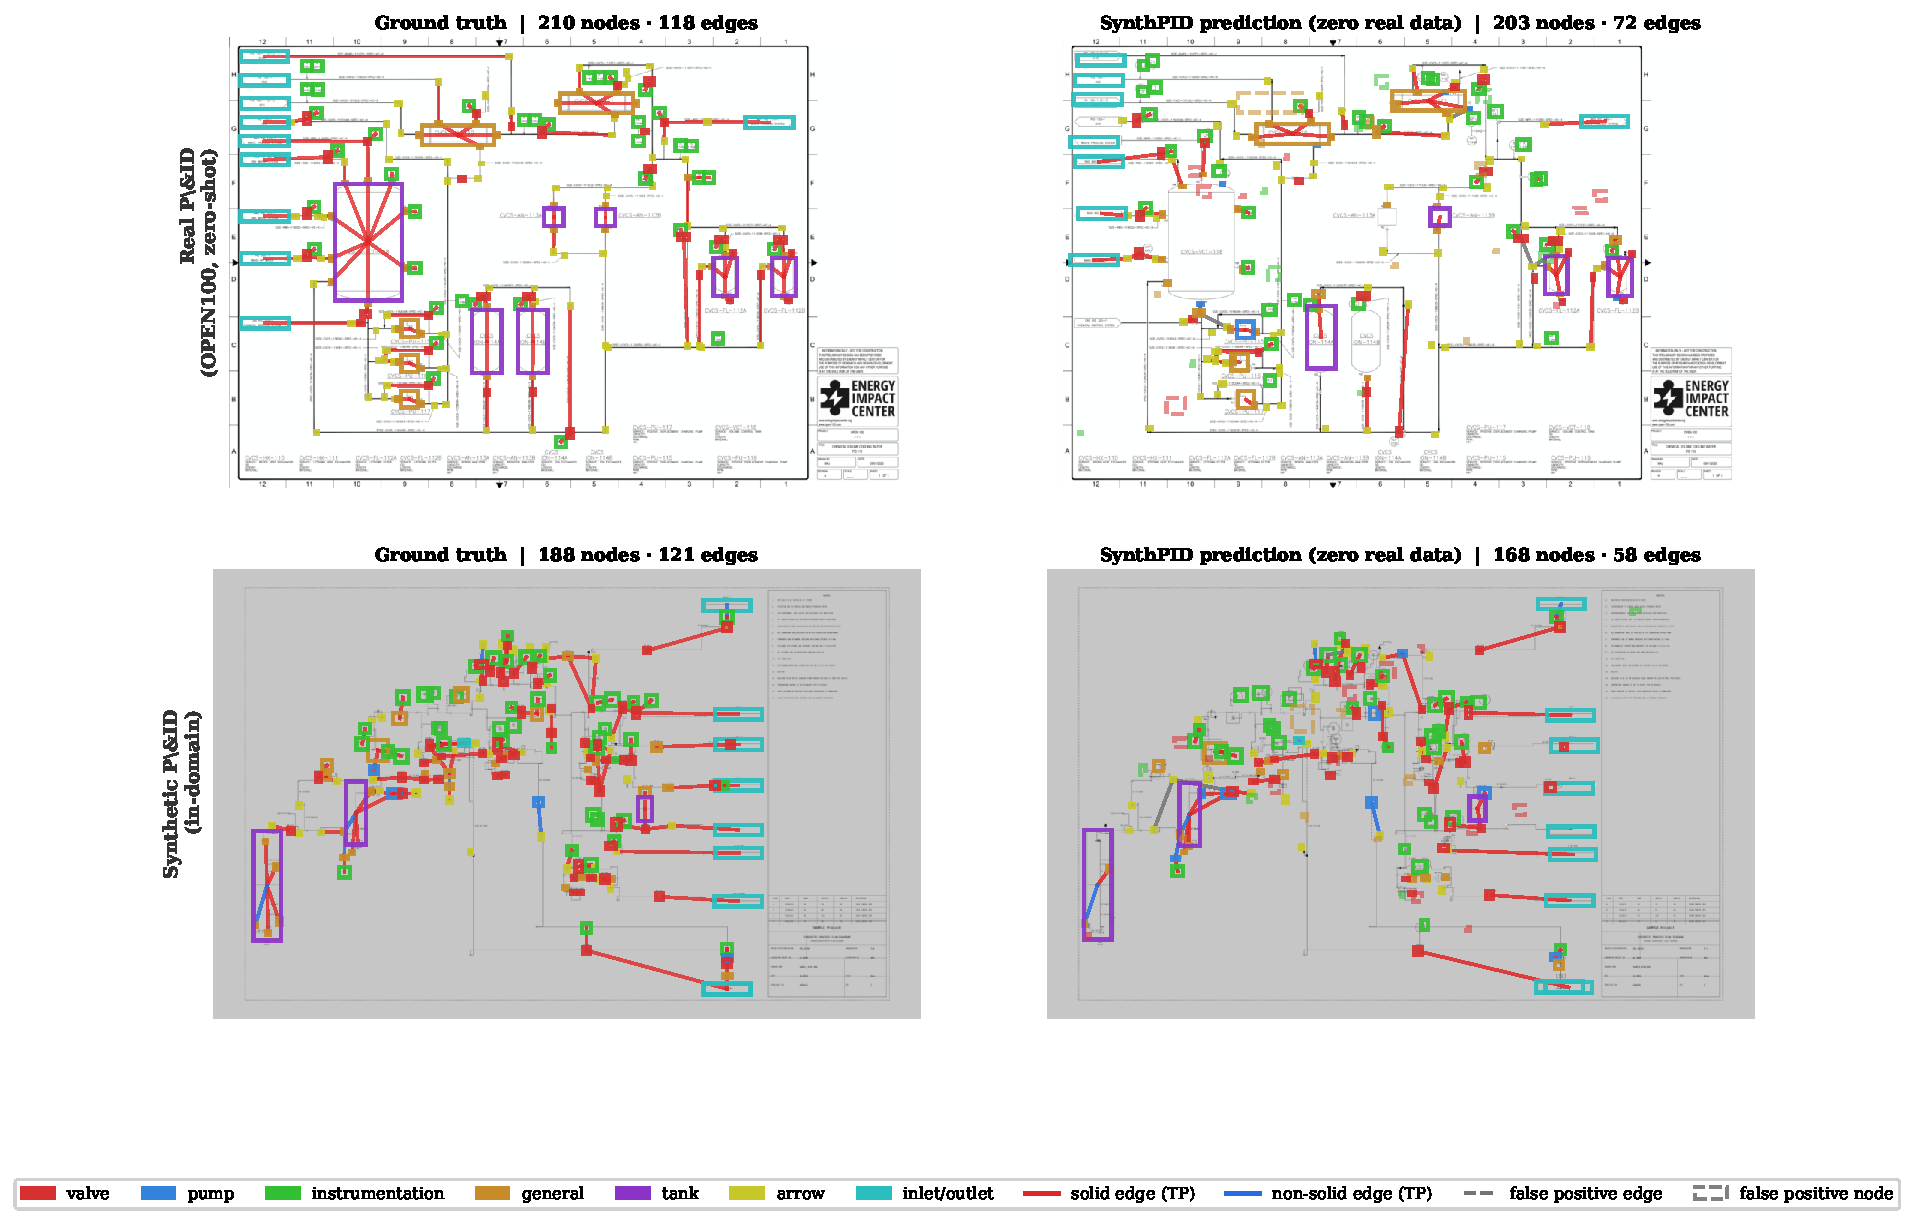
\includegraphics[width=\linewidth]{figures/qualitative_results.pdf}
    \caption{
        Ground truth (left) vs.\ \ours{} predictions (right) on a real
        OPEN100 P\&ID (top, zero real training data) and a synthetic
        \ours{} P\&ID (bottom, in-domain).
        Solid/dashed bounding boxes denote true-positive / false-positive
        node detections; solid/dashed edge lines denote TP/FP edges.
        The model recovers the majority of physical components and pipe
        connections; remaining errors concentrate on the \textit{general}
        class and densely packed regions.
    }
    \label{fig:qualitative}
\end{figure*}
